\subsection{Research Objectives}

%\begin{figure}[t]
%    \centering
%    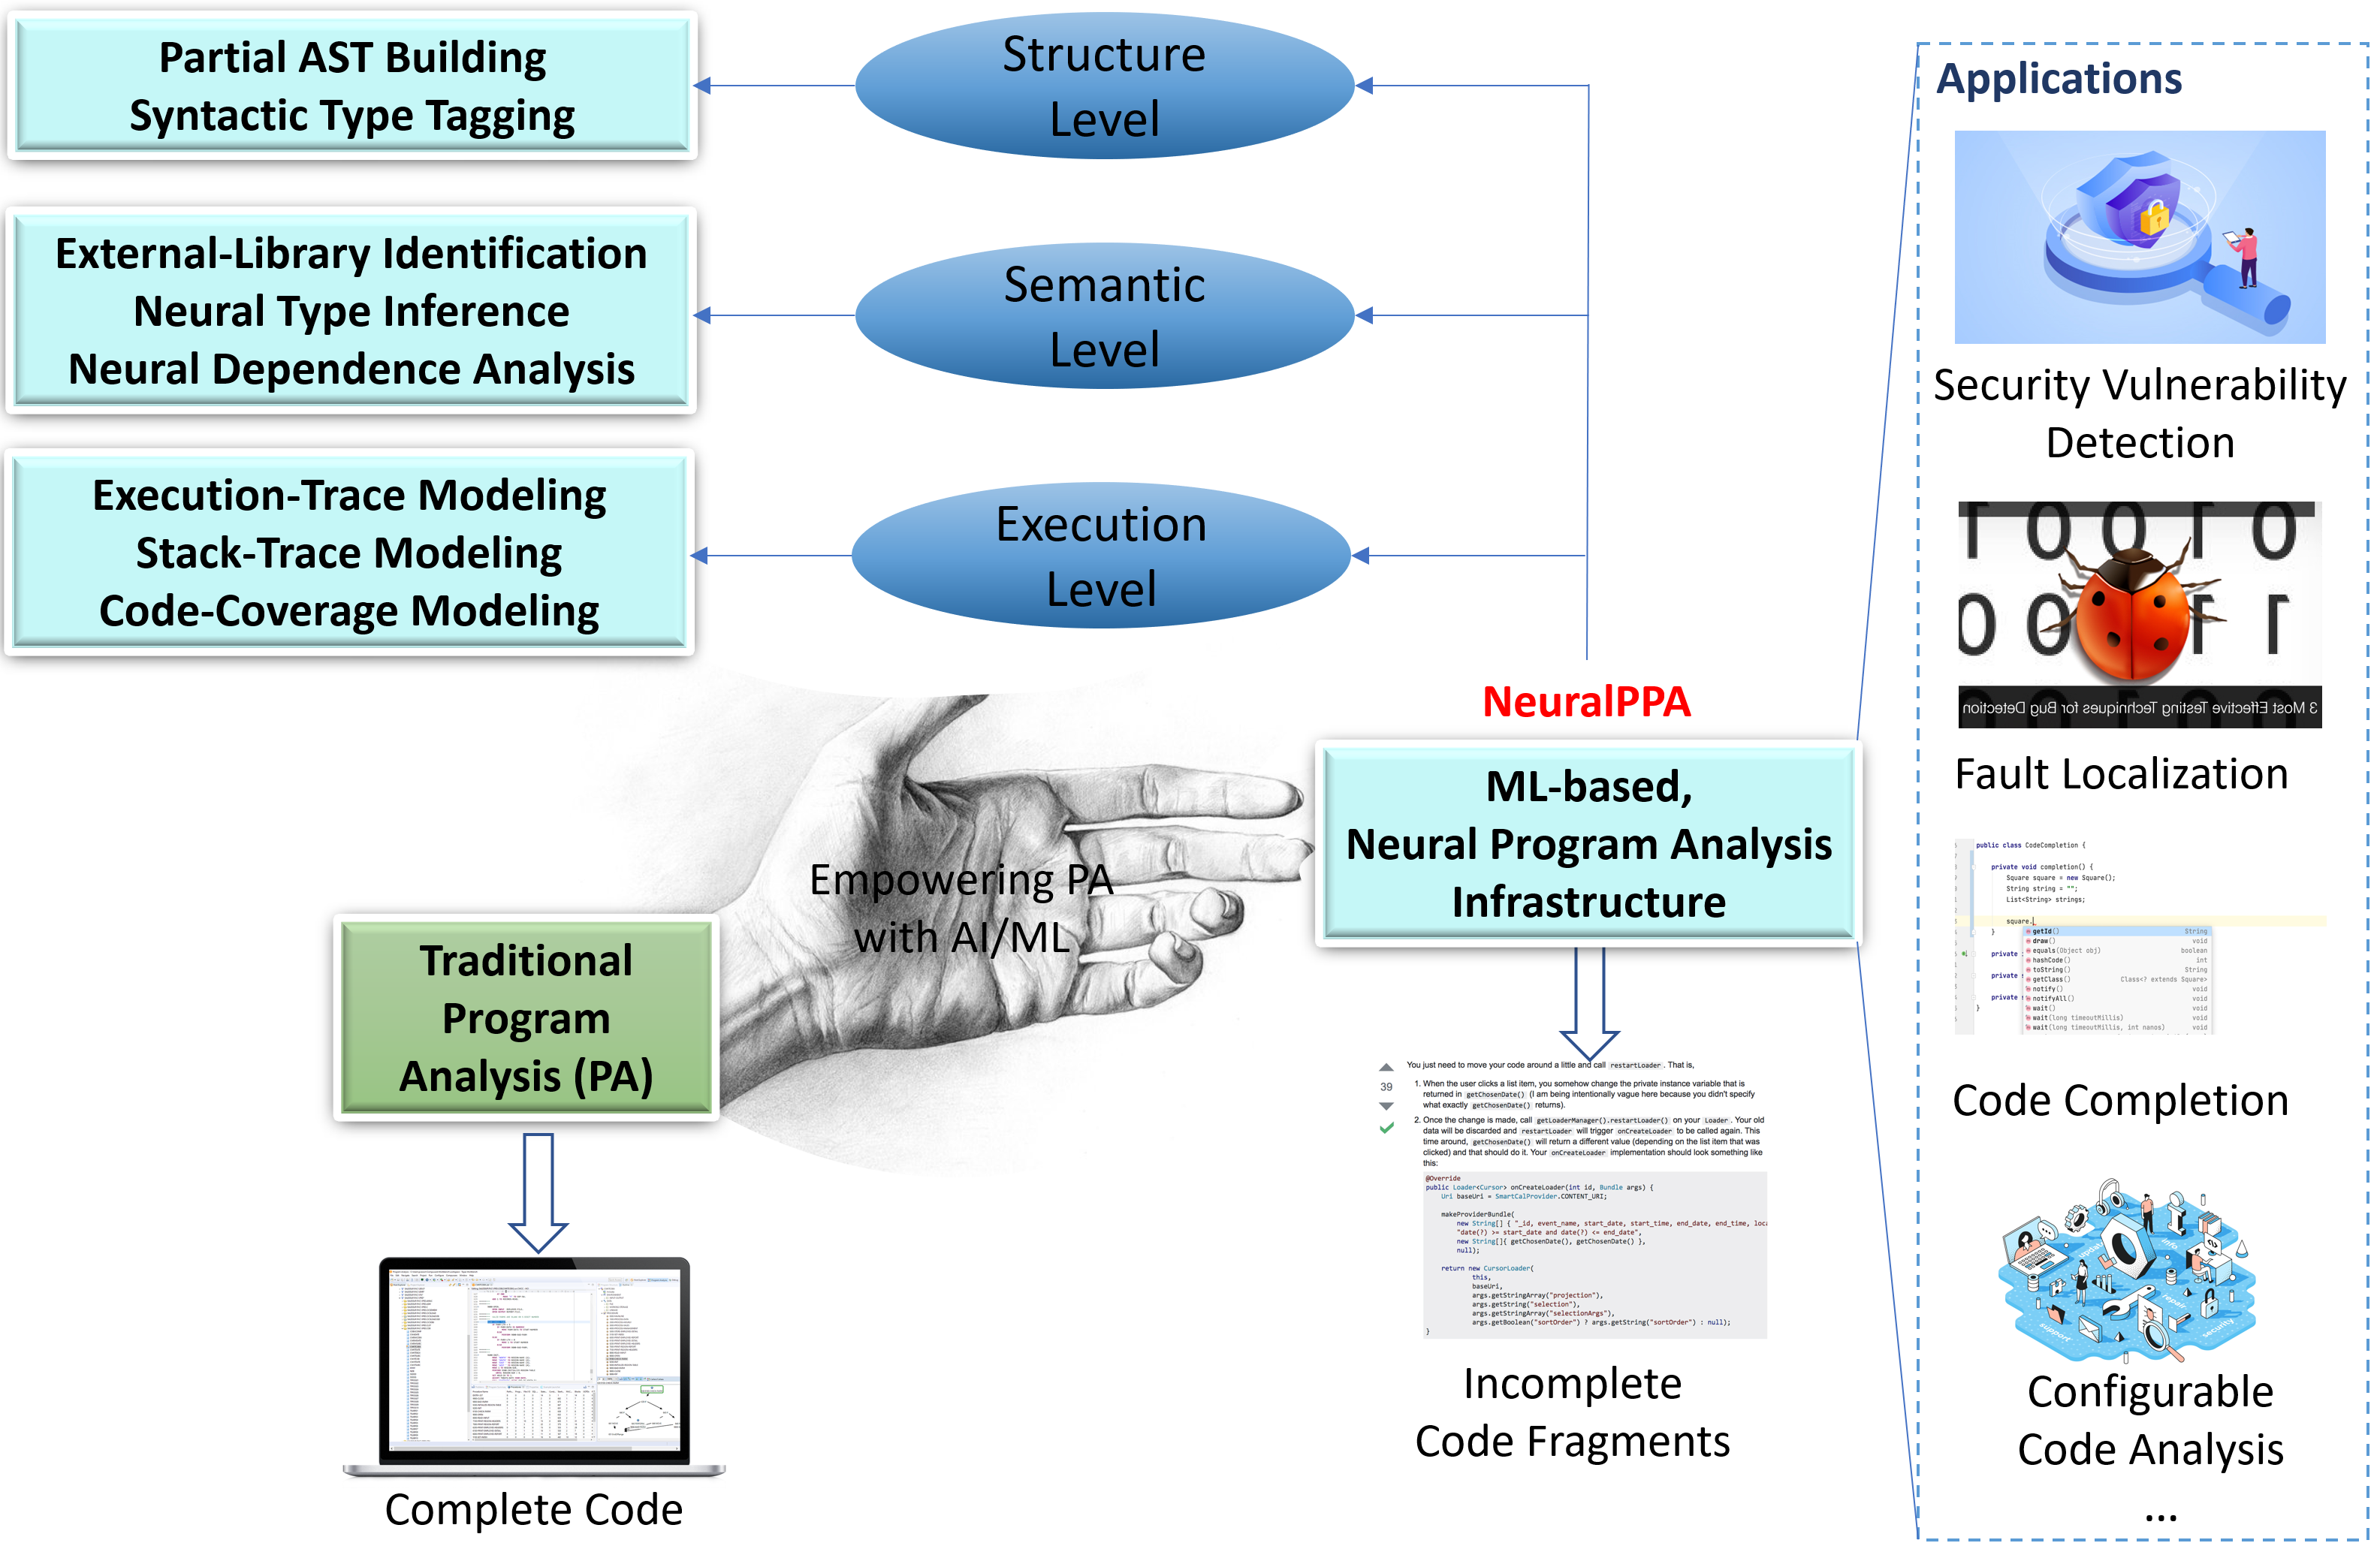
\includegraphics[width=0.83\textwidth]{graphs/neuralppa}
%    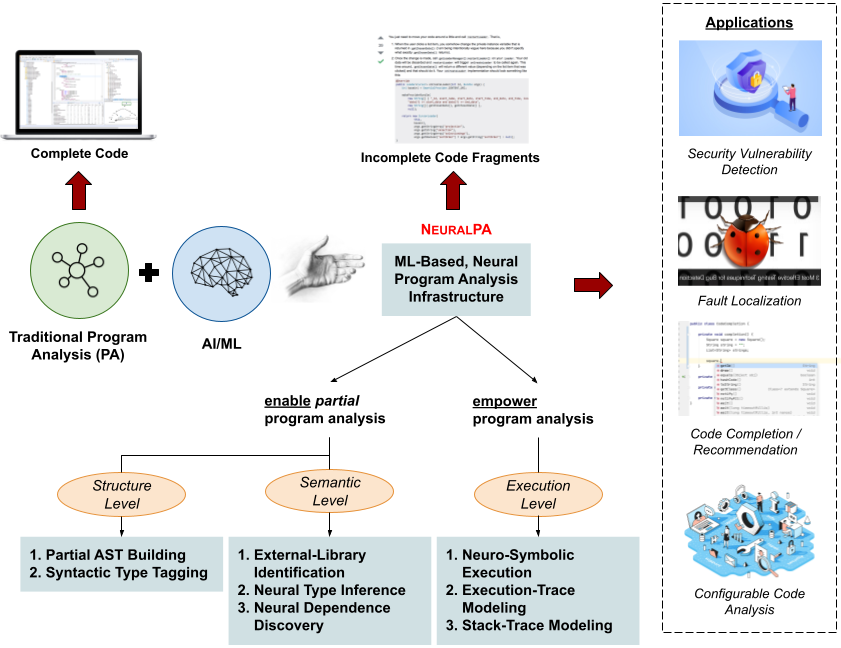
\includegraphics[width=0.92\textwidth]{figures/infra-design-3.png}
%    \vspace{-10pt}
%    \caption{{\tool}: Machine Learning-based Program Analysis Infrastructure}
%    \label{fig:arch}
%\end{figure}

In this proposal, we seek to create a paradigm shift in assisting the
visually-impaired programmers and learners with a Voice-to-Code
framework. We aim to establish {\em a scientific foundation, novel
  methodologies, frameworks, models, and algorithmic solutions for
  Voice-to-Code assistive technology}.

To address the above issues with the current assistive technology for
visually-impaired programmers and learners (VIPLs), we are embarking
on the development of a groundbreaking framework that leverages voice
interaction and advanced AI technologies.

{\bf Enabling Voice-Driven Interaction}: Our primary objective is to
empower visually-impaired programmers and students to interact
seamlessly with an IDE through the power of voice. This means that
instead of relying solely on audio cues, they will be able to
communicate their coding instructions and commands using spoken
language. By doing so, we aim to bridge the accessibility gap and
provide an intuitive and efficient way for visually-impaired
individuals to engage with programming tasks.

{\bf Voice-to-Text Conversion}: In our framework, the spoken word
becomes a bridge to the digital realm. We utilize state-of-the-art
voice recognition technology to accurately convert spoken language
into text. This initial step is crucial in translating the user's
voice commands and instructions into a format that can be further
processed by the system. This ensures that the users' intent is
accurately captured and preserved throughout the programming process.

{\bf Text-to-Code Generation with Generative AI}: Upon converting
voice inputs into textual form, we introduce the power of generative
artificial intelligence (AI). A large language model (LLM) with
generative capabilities takes the converted text and transforms it
into actual code. This step involves understanding the context,
syntax, and semantics of the instructions, and generating
corresponding code segments. The AI's ability to comprehend natural
language ensures that the generated code aligns with the user's
intentions.

{\bf Code Playback for Verification}: An integral aspect of our
framework is ensuring that the generated code is faithful to the
user's input. After the AI generates the code, it is read back to the
user through synthesized speech. This auditory feedback mechanism
enables visually-impaired programmers and students to verify the
accuracy of the generated code. By engaging their sense of hearing,
users can catch any discrepancies or errors and provide timely
corrections.

  
{\bf Empowering Modifications and Iterations}: Flexibility and control
are central to our framework's design. The visually-impaired users
have the ability to modify and refine the generated code according to
their preferences and needs. Through voice commands or text-based
interactions, they can make alterations, experiment with different
approaches, and fine-tune the code to align with their coding
goals. This iterative process ensures that the users are active
participants in the programming tasks.

In summary, our innovative framework for visually-impaired programmers
and learners offers a transformative way to engage with programming
tasks. By harnessing the capabilities of voice recognition, generative
AI from LLMs, and auditory feedback, we are working to create an
environment that fosters inclusivity, creativity, and
empowerment. Through this initiative, we aspire to break down barriers
and make the world of coding accessible to all, regardless of visual
impairments, contributing to a more diverse and vibrant programming
community.

\subsection{Thrusts of Research}

We propose the following thrusts of research in {\tool} (see Table~\ref{tab:milestones}):

\vspace{3pt}
%\noindent \textbf{Thrust 1. Neural Structural Analysis Infrastructure
%  \code{NeuralStruct}.} ({\em Section~\ref{}}) Source code has
%well-defined structures and semantics. Thus, the basic infrastructure
%in {\tool} is the neural structural analysis component.  This
%component has two main tasks. First, it learns from the syntactic
%structures of the complete code in the training dataset collected from
%large-scale code repositories, to derive the abstract syntax tree
%(AST) that best represents the syntactic structure of the given
%partial code, i.e., with the highest likelihood/probability.  The
%traditional lexical analyzer still works for partial code due to the
%independence nature of lexical tokens. The second task of this
%component is to tag the code tokens with the types of the syntactic
%units including the statement types (\code{if}, \code{for}, etc.),
%variables, fields, methods, classes, etc. Both of the tasks can be
%performed with our learning-based approaches in a dual-learning
%manner.

\noindent \textbf{Thrust 1. Empirical Study on Current Assistive
  Technology for VIPLs} ({\em Section~\ref{sec:thrust1}}) In order to
gain deeper insights into the challenges faced by visually-impaired
programmers and students in utilizing current assistive technologies
for programming or learning to program, we conducted an empirical
study. This study involved engaging a diverse group of
visually-impaired individuals with varying levels of programming
experience. Through in-depth interviews, surveys, and usability
testing, we aimed to uncover the specific pain points, limitations,
and usability issues encountered when utilizing existing assistive
tools in programming contexts. Participants were encouraged to share
their personal experiences, frustrations, and suggestions for
improvement. By systematically analyzing the data collected from this
study, we sought to identify common themes, technical obstacles, and
areas where assistive technologies fell short in meeting the unique
needs of visually-impaired individuals in the programming
domain. Ultimately, this empirical study serves as a foundational step
toward informing the development of more effective and inclusive
assistive technologies that cater to the diverse requirements of
visually-impaired programmers and students.



\vspace{3pt}
\noindent \textbf{Thrust 2. Voice-Driven Programming Framework for
  VIPLs.}  ({\em Section~\ref{sec:thrust2}}) Our initiative focuses on
empowering visually-impaired programmers and students by enabling them
to seamlessly interact with an integrated development environment
(IDE) through voice commands. Rather than relying solely on auditory
cues, this approach allows them to articulate coding instructions and
commands using spoken language, effectively bridging the accessibility
gap and providing an intuitive means for engaging with programming
tasks. Through cutting-edge voice recognition technology, spoken
language is converted into text, serving as a crucial initial step in
translating users' voice inputs into a processable format.

Subsequently, our framework integrates generative artificial
intelligence (AI) to facilitate the transformation of text back into
code. A sophisticated language model with generative capabilities
processes the textual input, considering the nuances of context,
syntax, and semantics to generate corresponding code segments that
accurately align with the users' intentions. To ensure the accuracy of
the generated code, our framework employs auditory feedback, where the
AI-generated code is read aloud to the user. This feedback mechanism
allows visually-impaired programmers and students to verify the code's
precision through their sense of hearing, enabling them to promptly
identify errors and discrepancies.

Central to our design is the empowerment of users through flexibility
and control. Visually-impaired individuals can actively modify and
refine the generated code to suit their preferences and coding
goals. This adaptability is facilitated through voice commands or
text-based interactions, allowing for alterations, experimentation
with diverse approaches, and fine-tuning of the code. This iterative
process ensures that users remain engaged and actively involved in the
programming tasks, ultimately fostering a sense of ownership and
inclusivity in their coding journey.

\vspace{3pt}
\noindent \textbf{Thrust 3. Voice-Driven Features for an IDE to
  support VIPLs.} ({\em Section~\ref{sec:thrust3}}) Introducing a
revolutionary programming environment tailored to the needs of
visually-impaired individuals, our cutting-edge platform offers a
multifaceted approach to programming through seamless voice
interaction. At the core of this environment lies direct communication
with ChatGPT, a sophisticated language model, which serves as a
personalized programming assistant. Users can articulate their
programming tasks through natural language voice commands, receiving
real-time feedback, suggestions, and guidance to navigate coding
challenges effectively. This feature not only democratizes the
programming experience but also empowers visually-impaired programmers
to engage in a more intuitive and productive coding process.

Our programming environment goes beyond voice interaction by enabling
the transformation of voice commands into tangible code. Leveraging
advanced voice recognition and generative AI technologies, users'
spoken instructions are converted into actual code snippets. This
bridges the gap between verbal expression and code creation, ensuring
that the users' intent is accurately translated into executable code
segments. The generated code is then read back to the users through
synthesized speech, allowing them to verify its accuracy and
completeness, while promoting a understanding of the
programming logic.

This innovative environment extends its functionality to seamlessly
integrate generated code with existing projects, simplifying the
collaborative process and enabling a cohesive workflow. In addition,
users can harness the power of voice to initiate debugging sessions,
identifying and rectifying errors through intuitive voice
commands. The environment also facilitates the generation of
comprehensive documentation, providing a holistic overview of the
codebase, which can be enriched and customized through voice
interactions. Furthermore, users can effortlessly create test cases
using voice commands, enhancing the testing and validation of their
code. By encompassing these features, our programming environment
empowers visually-impaired programmers with a versatile and inclusive
toolset, fostering a dynamic programming journey while mitigating
accessibility barriers.


%1) Voice interaction with ChatGPT on programming tasks

%2) Code Generation from Voice

%3) Reading back the generated code for verification

%4) Code integration with existing code

%5) Debugging code via Voice Commands

%6) Documentation generation

%7) Test case generation


%\vspace{3pt}
%\noindent \textbf{Thrust ???. Neural Execution Analysis Infrastructure.}
%({\em Section~\ref{}}) All the dynamic analysis techniques require the
%analysis and understanding of the execution. However, for an
%incomplete code, we first need to design a component that can wrap
%around the given code fragment with the minimum code so that the code
%fragment can be executed. When the code is executed, we also need the
%approaches that represent the executed statements and their relations,
%model the execution and stack traces, and model the code coverages
%for an execution.

\begin{table*}[t]
	\vspace{-15pt}
\begin{center}
{\footnotesize{
\begin{tabular}{cc}
\begin{tabular}[t]{|p{0.2in}|p{2.95in}|} 
\hline
\multicolumn{2}{|>{\columncolor[gray]{0}}c|}{\textcolor{white}
{\bf Year 1 Project Milestones \& Deliverables}}\\
\hline 
\hline
\multicolumn{2}{|c|}{\bf T1. Neural Structure Analysis Infrastructure}\\
\hline
{\bf 1.1} & Neural Syntactic Type Tagging\\
{\bf 1.2} & Neural Partial AST Building\\
{\bf 1.3} & Evaluation of the components\\
\hline
\hline
\multicolumn{2}{|c|}{\bf T2. Neural Semantic Analysis Infrastructure}\\ 
\hline
{\bf 2.1} & External-Library Identification\\
\hline
%\hline
%\multicolumn{2}{|c|}{\bf Integrate Code Synthesis into Tools}\\
%\hline
%{\bf 1.5} & \goalOneFour.\\
%\hline
\multicolumn{2}{c}{}
\end{tabular}
&
\begin{tabular}[t]{|p{0.2in}|p{2.95in}|} \hline
\multicolumn{2}{|>{\columncolor[gray]{0}}c|}{\textcolor{white}
{\bf Year 2 Project Milestones \& Deliverables}}\\
\hline 
\hline
\multicolumn{2}{|c|}{\bf T2. Neural Semantic Analysis Infrastructure}\\
\hline
{\bf 2.2} & Neural Type Inference\\
{\bf 2.3} & Neural Dependence Analysis\\
%{\bf 2.3} & Integrate Evaluation Framework into Design Environment\\
%{\bf 2.4} & Evaluate CRL Framework with Existing Models\\
%{\bf 2.3} & \goalTwoThree.\\

\hline
\hline
\multicolumn{2}{|c|}{\bf T3. Neural Execution Analysis}\\ 
\hline
%{\bf 3.1} & Design New Code Representations and Learning Models.\\
{\bf 3.1} & Neural Execution-Trace Modeling\\
%{\bf 2.4} & Advance FL and RT-CI Approaches.\\
%{\bf 2.5} & Advance Regression Testing in CI Approaches.\\
%{\bf 2.5} & Advance APR Approaches with Framework.\\
\hline
%\hline
%\multicolumn{2}{|c|}{\bf Community Involvement: Capacity Building}\\
%\hline
%{\bf 2.4} & \goalTwoFour.\\
%{\bf 2.5} & \goalTwoFive.\\
%{\bf 2.6} & \goalTwoSix.\\
%\hline
\multicolumn{2}{c}{}
\end{tabular}
\end{tabular}\\
\vspace*{-.3cm}
\begin{tabular}{c}\hline
\multicolumn{1}{|>{\centering\columncolor[gray]{0}}p{6.44in}|}{\textcolor{white}
{\bf Year 3 Project Milestones \& Deliverables}}\\
\hline
\end{tabular}\\
\vspace*{-.2cm}
\begin{tabular}{cc}
\begin{tabular}[t]{|p{0.2in}|p{2.95in}|}
\hline
\multicolumn{2}{|c|}{\bf T3. Neural Execution Analysis}\\
\hline
{\bf 3.2} & Neural Stack Trace Modeling\\
{\bf 3.3} & Neural Code Coverage Modeling\\

%{\bf 3.3} & Testing on Models in IDE tools.\\
\hline
%\hline
%\multicolumn{2}{|c|}{\bf \goalTwo}\\ 
%\hline
%{\bf 3.3} & \goalThreeThree.\\
%\hline
\multicolumn{2}{c}{}
\end{tabular}
&
\begin{tabular}[t]{|p{0.2in}|p{2.95in}|}
\hline
\multicolumn{2}{|c|}{\bf T4. Neural Partial Program Analysis Applications}\\
\hline
%{\bf 3.1} & Design New Code Representations\\

{\bf 4.1} & Security Vulnerablity Detection with {\tool}\\
{\bf 4.2} & Fault Localization and Completion with {\tool}\\

\hline
\multicolumn{2}{c}{}
\end{tabular}
\end{tabular}
\vspace{-15pt}
}}
\end{center}
\vspace*{-.3in}
%\caption{Tasks and Milestones. (Rep. = Representation)}
\caption{The 3-year schedule of Thrusts, Tasks, and Milestones of this proposal.}
%the schedule of Thrusts, Tasks, and Milestones of this proposal.
%\vspace{-10pt}
\label{tab:milestones}
\vspace{-10pt}
\end{table*}
%

